\documentclass[11pt,letterpaper]{article}
\usepackage[margin=1in]{geometry}
\usepackage{amsmath,amssymb}
\usepackage{graphicx}
\usepackage{booktabs}
\usepackage{tabularx}
\usepackage{array}
\usepackage{xurl}
\usepackage{hyperref}
\usepackage[numbers,sort&compress]{natbib}
\usepackage{setspace}
\usepackage{caption}
\usepackage{float}
\usepackage{xcolor}
\hypersetup{colorlinks=true,linkcolor=blue!60!black,citecolor=blue!60!black,urlcolor=blue!60!black}
\captionsetup{font=small,labelfont=bf}
\usepackage{microtype}
\setstretch{1.15}
\emergencystretch=1.5em

\title{\textbf{Allele-Exact, Ploidy- and Denominator-Controlled Cross-Ancestry Audit of ClinVar Across All 84 ACMG SF v3.3 Genes Under gnomAD v4.1: Pipeline Artifacts, Recessive Return Hazards, and Verified ClinGen CSpec / DAFT VUS Frequency Conflicts}}
\author{Autonomous Computational Genomics Audit\\
\small Study A-1: Revised Post-Forensic Audit, Live ClinGen CSpec \& chrX Ploidy Verification,\\
\small and Prospective 20-Gene Out-of-Sample Validation\\
\small Snapshots: ClinVar GRCh38 (2026-11-24) $\times$ gnomAD v4.1 (807,162) $\times$ CSpec (2026-11-25)}
\date{November 25, 2026}

\begin{document}
\maketitle

\begin{abstract}
\noindent\textbf{Background:} Clinical sequencing laboratories rely on ClinVar classifications across the 84 medically actionable genes in ACMG SF v3.3 to guide preventive surgery, cardiac device implantation, and cascade testing. While gnomAD v4.1 expands reference variation to 807,162 individuals and Johnston et al.\ (2026) recently established disease allele frequency thresholds (DAFTs) across secondary-finding genes, automated ClinVar--gnomAD audits remain vulnerable to multiallelic rsID join collisions, unequal ancestry allele-number denominators, chrX non-PAR ploidy mis-filtering, stealth technical QC failures, and unstratified recessive-versus-dominant ClinVar VCF tags.

\noindent\textbf{Methods:} We joined all 343,328 ClinVar GRCh38 variants across all 84 ACMG SF v3.3 genes to all 545,493 gnomAD v4.1 variants using exact minimal representation (\path{CHROM-POS-REF-ALT}; $n=155,434$ matched variants; independent API $\mathrm{FAF}_{95}$ correlation $r=0.9997$). We enforced ploidy- and PAR-aware callability ($\mathrm{AN}\ge 80\%$ of $2N=1,614,324$ on autosomes/PAR, and of official $N_{XY}+2N_{XX}=400,897+2\times 406,265=1,213,427$ on non-PAR chrX covering \textit{ABCD1}, \textit{GLA}, and \textit{OTC}) and extracted exome+genome hemizygote counts. We controlled cross-ancestry denominator bias via $\mathrm{FAF}_{95}\ge 10^{-4}$ ($n=10,058$), $\mathrm{AC}\ge 10$ filters ($n=4,932$), and exact equal-AN hypergeometric downsampling ($\mathrm{AN}_{\mathrm{NFE}}=\mathrm{AN}_p$). To guarantee 100\% primary-source threshold traceability, we retrieved all 250 live ClinGen Criteria Specification Registry (CSpec) SVI JSON documents (2026-11-25) and combined the 30 officially Released ACMG SF v3.3 VCEP specifications (including \textit{OTC} \texttt{GN156} v1.0's $\ge 10$ homozygote/hemizygote BA1 criterion) with Johnston et al.'s (2026) published preliminary VCEP (6 genes) and DAFT BS1/BA1 thresholds (47 genes; excluding single-variant \textit{HFE} and named BA1/BS1 exceptions). We live-audited 100\% (55/55) of allele-exact 2--4$\star$ AD P/LP alerts and 100\% (18/18) of flagged X-linked alerts against gnomAD v4.1 exome/genome QC filters, evaluated VUS persistence using collapsible linear probability models (LPM) and non-parametric submitter-tier stratification, and executed a prospectively locked out-of-sample validation across 20 unseen autosomal AD genes (99,249 ClinVar $\times$ 157,021 gnomAD v4.1; $n=38,023$ exact matches).

\noindent\textbf{Results:} First, naive rsID joins inflate P/LP frequency alerts ($\mathrm{FAF}_{95}\ge 10^{-4}$) by 72.2\% overall (544 vs.\ 151 exact) and 79.7\% among 2--4$\star$ AD alerts (271 vs.\ 55 exact), replicating at 84.6\% / 80.2\% in the 20 unseen genes. Second, raw $\mathrm{AF}\ge 10^{-4}$ screening induces a spurious aggregate P/LP disparity driven by 64.7\% singletons ($\mathrm{AC}=1$) in small-AN Middle Eastern samples (median $\mathrm{AN}=6,006$ vs.\ NFE $1,179,788$); under ploidy- and denominator-clean $\mathrm{FAF}_{95}\ge 10^{-4}$ ($n=10,058$) and equal-AN hypergeometric downsampling, aggregate P/LP disparity collapses to null or reverses (CMH $\mathrm{OR}=1.55$, $p=0.391$; hypergeometric ORs $0.42$--$1.27$; unseen 20-gene $\mathrm{OR}=0.36$, $p=0.169$). Conversely, non-European VUS persistence survives every clean test (ACMG 84 ploidy-aware: 12.01\% vs.\ 6.86\%, CMH $\mathrm{OR}=2.62$, $p=2.03\times 10^{-9}$; collapsible LPM $+8.86$ pp, $p=1.96\times 10^{-17}$; hypergeometric ORs $1.62$--$2.72$, all $p\le 1.3\times 10^{-5}$; unseen 20-gene LPM $+10.84$ pp, $p=5.93\times 10^{-6}$). Within every fixed submitter-count tier ($1$, $2$--$3$, $4$--$9$, $10$--$19$, $20+$), non-NFE and NFE VUS rates are indistinguishable (all Fisher $p\ge 0.16$); conditioning on submitter-tier bins descriptively attenuates the LPM gap by 55.5\% (unseen 20-gene: 50.0\%), though cross-sectional adjustment cannot identify causal mediation. Third, complete live-QC, official CSpec/DAFT, and mode-of-inheritance triage of all 55 allele-exact 2--4$\star$ AD alerts yields \textbf{0/55} exceeding verified BA1 and \textbf{0/55} unambiguous frequency-only AD P/LP misclassifications: 8/55 (14.5\%) are gnomAD QC/callability artifacts (including stealth \texttt{AS\_VQSR} failure in \textit{APC} c.423-3T$>$A at 93.9\% AN), 22/55 (40.0\%) FIN/ASJ bottleneck founders, 14/55 (25.5\%) established continental founders/reduced-penetrance alleles, 6/55 (10.9\%) genuine AD alleles strictly below verified BS1, 1/55 (1.8\%) reduced-penetrance \textit{CACNA1S} p.Arg1086Ser above Johnston DAFT BS1 but below BA1, and 4/55 (7.3\%) recessive myopathy alleles in dual-mode \textit{RYR1}/\textit{TTN} creating an AR-in-AD VCF return hazard (with ClinGen CSpec \texttt{GN179} explicitly listing \textit{RYR1} c.10348-6C$>$G as an AR myopathy BA1/BS1 exclusion). Fourth, fixing autosomal-vs-chrX ploidy filtering recovers 406/441 X-linked VUS (\textit{ABCD1} 200/207, \textit{GLA} 117/137, \textit{OTC} 89/97) and yields \textbf{327 high-callability VUS $\ge$ official BS1/BA1} (77.7\% NFE-invisible; 278 with $\mathrm{AC}\ge 5$) and \textbf{21 $\ge$ BA1} (90.5\% NFE-invisible) strictly within the 30 Released CSpec VCEP genes---including 11 \textit{ABCD1} (\texttt{GN105}; 1 above BA1 with 17 hemizygotes, 1 \texttt{AS\_VQSR}+\texttt{segdup} fail, 4 \texttt{segdup}-flagged) and 5 \textit{OTC} VUS meeting \texttt{GN156}'s $\ge 10$ male-hemizygote BA1 criterion (12--55 hemizygotes, 5/5 live-QC PASS)---plus 99/9 in 6 preliminary VCEP genes and 962/216 in 47 Johnston DAFT genes (1,388 total $\ge$ BS1/BA1, 246 $\ge$ BA1 across 51,190 high-callability VUS; combined live QC audit: 36/37 = 97.3\% PASS).

\noindent\textbf{Conclusions:} Extending Johnston et al.'s (2026) DAFT baseline with live 2026 CSpec specifications, ploidy-correct chrX callability and hemizygote parsing, allele-exact QC auditing, and denominator-controlled ancestry modeling shows that high-confidence (2--4$\star$) AD P/LP assertions are far cleaner than naive audits imply. Clinical pipelines should prioritize (i) allele-exact joins with mandatory gnomAD filter gating and ploidy-aware chrX denominators, (ii) mode-of-inheritance tags in ClinVar VCF exports for dual-mode genes, and (iii) formal VCEP re-evaluation of the 327 CSpec-governed VUS frequency-conflict candidates heavily enriched in non-European ancestries.
\end{abstract}

\section{Introduction}
The American College of Medical Genetics and Genomics Secondary Findings v3.3 policy statement (ACMG SF v3.3) recommends opportunistic clinical return of Pathogenic and Likely Pathogenic (P/LP) variants across 84 medically actionable genes encompassing hereditary cancer syndromes, cardiomyopathies, arrhythmias, aortopathies, metabolic disorders, and pharmacogenetic malignant hyperthermia \citep{lee2025acmg,miller2023acmg}. Clinical interpretation relies heavily on ClinVar \citep{landrum2025clinvar} coupled with population reference allele frequencies under the ACMG/AMP framework \citep{richards2015standards}, refined by Whiffin et al.'s maximum credible population allele frequency ($\mathrm{FAF}_{95}$) framework \citep{whiffin2017frequency} and ClinGen Sequence Variant Interpretation (SVI) guidance \citep{ghosh2018ba1}.

A decade ago, Manrai et al.\ demonstrated that limited ancestral diversity in reference cohorts caused benign African-ancestry variants to be misclassified as pathogenic in hypertrophic cardiomyopathy \citep{manrai2016misdiagnoses}, alongside broad inequities in Variant of Uncertain Significance (VUS) rates \citep{popejoy2016diversity,caswelljin2018disparities}. The release of gnomAD v4.0/v4.1---aggregating 807,162 individuals (730,947 exomes and 76,215 genomes; 406,265 XX and 400,897 XY samples) with joint allele numbers across all called sites \citep{gnomadv41release2024,gnomadv41sex2024}, building upon gnomAD v2 \citep{karczewski2020gnomad} and gnomAD v3.1.2 \citep{chen2024gnomadv3}---markedly increased non-European sample sizes.

Recent studies have leveraged gnomAD v4 alongside ClinVar across complementary clinical domains. Table~\ref{tab:prior_art} provides a direct side-by-side comparison with six closest prior studies and specifies our incremental contributions. Most closely, Johnston et al.\ (2026) compiled ClinGen VCEP BA1/BS1 rules as of June 15, 2025 (28 approved + 8 preliminary) and derived disease allele frequency thresholds (DAFTs; $\mathrm{BS1}=\mathrm{DAFT}$, $\mathrm{BA1}=10\times\mathrm{DAFT}$) for 58 remaining monogenic disease entities (47 genes) across ACMG SF v3.3 (83 genes excluding single-variant \textit{HFE}), validating them against ClinVar P/LP and novel pLoF variants and observing zero P/LP variants above BA1 and nine above BS1 \citep{johnston2026daft}. Gudmundsson et al.\ manually audited 734 pLoF variants across 77 severe early-onset haploinsufficient genes in 807,162 gnomAD v4 individuals \citep{gudmundsson2025penetrance}. Hotakainen et al.\ estimated recessive carrier frequencies in gnomAD v4.0 \citep{hotakainen2025carrier}. In 2026, Dario analyzed annotation coverage across 16 monogenic diabetes genes \citep{dario2026mody}, Lai et al.\ audited EAS-vs-NFE P/LP variants across 199 epilepsy genes while quantifying a 75.0\% false-positive rate from rsID-level joins \citep{lai2026epilepsy}, and Ernest \& Ansah audited 32 kidney-disease genes with allele-number equalization sensitivity checks \citep{ernest2026kidney}.

\begin{table}[H]
\centering
\caption{Side-by-Side Comparison with Closest Published gnomAD v4 $\times$ ClinVar Studies.}
\label{tab:prior_art}
\scriptsize
\setlength{\tabcolsep}{4pt}
\begin{tabularx}{\textwidth}{>{\raggedright\arraybackslash}p{2.5cm}>{\raggedright\arraybackslash}p{2.6cm}>{\raggedright\arraybackslash}p{3.2cm}>{\raggedright\arraybackslash}X}
\toprule
\textbf{Study} & \textbf{Gene Scope \& Data} & \textbf{Primary Focus} & \textbf{Distinct Additions in Present Study} \\
\midrule
Johnston et al., \textit{Genet Med} 28(5):102552 (2026) \citep{johnston2026daft} & 83 ACMG SF v3.3 genes (excl.\ \textit{HFE}); gnomAD v4.1; CSpec to Jun 2025 & Derives MDE-specific DAFT BS1/BA1; checks P/LP \& pLoF (0 $>$ BA1, 9 $>$ BS1) & Updates to live Nov 2026 CSpec (30 Released VCEPs incl.\ newly released \textit{ABCD1}/\textit{OTC} + hemizygote rule \& \textit{PMS2} v2.0); adds rsID FPR audit, equal-AN hypergeometric testing, ploidy-correct chrX callability, submitter-tier stratification, 55/55 live QC catch (\textit{APC} \texttt{AS\_VQSR}), AR-in-AD VCF hazard, 51,190-VUS BS1/BA1 queue, and 20 unseen AD genes. \\
Gudmundsson et al., \textit{Nat Commun} 2025 \citep{gudmundsson2025penetrance} & 77 early-onset haploinsufficient genes; gnomAD v4 (807k) & Case-by-case penetrance / rescue of 734 pLoF variants & Audits all 84 adult-actionable ACMG SF v3.3 genes (all coding/splice classes + VUS), rsID inflation, denominator bias, AR-in-AD VCF hazard, and 20 unseen AD genes. \\
Hotakainen et al., \textit{Genet Med} 2025 \citep{hotakainen2025carrier} & Recessive/XL carrier screening genes; gnomAD v4.0 & Carrier \& at-risk couple frequencies & Focuses on actionable AD/XL secondary findings, 55/55 live QC/CSpec triage, cross-ancestry VUS equity, and gene-specific BS1/BA1 VUS review queue. \\
Dario, \textit{Ann Hum Genet} 2026 \citep{dario2026mody} & 16 MODY diabetes genes; gnomAD v4.0 $\times$ ClinVar & Population-private annotation coverage \& P/LP vs.\ VUS & Multi-ancestry (6 groups) across 84 ACMG + 20 unseen AD genes; exact equal-AN hypergeometric downsampling; collapsible LPM \& submitter-tier stratification. \\
Lai et al., \textit{Front Genet} 2026 \citep{lai2026epilepsy} & 199 epilepsy genes; EAS vs.\ NFE in gnomAD v4.1.1 & EAS-enriched P/LP alleles; documented 75.0\% rsID FPR & Replicates 72.2\%--84.6\% rsID FPR across ACMG 84 \& unseen 20 genes; adds VUS disparity, singleton bias retraction, and live QC/CSpec audit. \\
Ernest \& Ansah, \textit{Res Sq} 2026 \citep{ernest2026kidney} & 32 kidney genes; gnomAD v4.1 + 421 West African genomes & AFR vs.\ NFE frequency ceilings \& AN equalization & Full ACMG SF v3.3 panel across 5 non-NFE ancestries, live CSpec + Johnston DAFT baseline, chrX ploidy fix, stealth \texttt{AS\_VQSR} catch, AR-in-AD hazard, and 20-gene prospective lock. \\
\bottomrule
\end{tabularx}
\end{table}

Crucially, during our forensic self-audit of our initial analysis plan (accurately labeled a Post-Pilot Analysis Plan; original timestamp \texttt{2026-11-25 08:45 CST}, preserved in \texttt{PREREG\_A1.md}), we uncovered and corrected four concrete pitfalls: (1) raw $\mathrm{AF}\ge 10^{-4}$ screens create an artificial aggregate P/LP disparity driven by singletons in small-AN ancestries; (2) uniform $\mathrm{FAF}_{95}\ge 10^{-4}$ flags without live gnomAD QC filter inspection and mode-of-inheritance parsing falsely label technical artifacts and recessive myopathy alleles as dominant misclassifications; (3) manually transcribed VCEP cutoffs (e.g., an earlier erroneous \textit{APC} BS1 of $10^{-4}$ instead of ClinGen InSiGHT \texttt{GN089} v2.0/v2.1's official $10^{-5}$ \citep{spier2024apc}) distort VUS counts by an order of magnitude; and (4) applying an autosomal $80\%$ allele-number callability cutoff ($1,291,459$) to non-PAR chrX genes (\textit{ABCD1}, \textit{GLA}, \textit{OTC}) silently excluded 100\% (441/441) of X-linked VUS because their true diploid+hemizygous maximum AN is $N_{XY}+2N_{XX}=1,213,427$ \citep{gnomadv41sex2024}. We corrected all four errors end-to-end and validated our cross-ancestry and rsID findings out-of-sample in a genuinely prospectively locked cohort of 20 unseen autosomal AD genes (\texttt{PROSPECTIVE\_VALIDATION\_A1.md}, locked \texttt{2026-11-25 09:51 CST} prior to data extraction).

\section{Methods}
\subsection{Data Sources, Allele-Exact Matching, Ploidy-Aware Callability, and $\mathrm{FAF}_{95}$ Verification}
We extracted all GRCh38 records for all 84 ACMG SF v3.3 genes (72 AD, 9 AR, 3 X-linked; 28 Cancer, 43 Cardiovascular, 5 Metabolic, 8 Miscellaneous) from NCBI ClinVar bulk FTP releases \texttt{clinvar.vcf.gz} (2026-11-24; 4,621,342 total rows; 343,328 in ACMG SF v3.3) and \texttt{variant\_summary.txt.gz} (2026-11-23; 100\% VariationID enrichment for \texttt{LastEvaluated} and \texttt{NumberSubmitters}). We retrieved all 545,493 gnomAD v4.1 (\texttt{gnomad\_r4}) variants across all 84/84 genes via the Broad Institute GraphQL API (with region-chunking fallback for ultra-large loci including \textit{TTN}), retaining exome and genome allele counts, allele numbers, homozygote counts, and chrX hemizygote counts. Variants were joined strictly on normalized minimal GRCh38 alleles (\path{CHROM-POS-REF-ALT}), yielding $155,434$ exact matches (62,889 B/LB, 55,608 VUS, 27,384 Conflicting, 8,962 P/LP, 589 Other, 2 P/LP low-penetrance).

All three X-linked ACMG SF v3.3 genes reside strictly outside GRCh38 pseudoautosomal regions (PAR1: \path{chrX:10,001-2,781,479}; PAR2: \path{chrX:155,701,383-156,030,895}): \textit{OTC} (\path{38.35-38.42 Mb}), \textit{GLA} (\path{101.40-101.41 Mb}), and \textit{ABCD1} (\path{153.73-153.74 Mb}). Using the official gnomAD v4.1 sex-karyotype sample counts (exomes: 367,323 XX + 363,624 XY = 730,947; genomes: 38,942 XX + 37,273 XY = 76,215; joint total: 406,265 XX + 400,897 XY = 807,162 \citep{gnomadv41sex2024}) and the \texttt{gnomad\_methods} non-PAR ploidy formula $\mathrm{AN}_{\max,\text{X-nonPAR}} = N_{XY} + 2 N_{XX}$, we define ploidy-aware high callability ($\ge 80\%$ of expected maximum AN) as:
\begin{itemize}
  \item \textbf{Autosomes and PAR1/PAR2:} $\mathrm{AN}_{\text{joint}} \ge 0.80 \times 1,614,324 = 1,291,459.2$.
  \item \textbf{chrX Non-PAR (\textit{ABCD1}, \textit{GLA}, \textit{OTC}):} $\mathrm{AN}_{\text{joint}} \ge 0.80 \times 1,213,427 = 970,741.6$ (empirically verified against the maximum observed joint AN of $1,211,320$ across all 6,997 cached chrX variants; zero variants differ between the exact official constant $1,213,427$ and an earlier site-ratio estimate $1,214,237$).
\end{itemize}
This recovers 406 of 441 X-linked VUS that were previously excluded (\textit{ABCD1}: 200/207 [96.6\%], \textit{GLA}: 117/137 [85.4\%], \textit{OTC}: 89/97 [91.8\%]), yielding $51,190$ high-callability VUS across all 83 thresholded genes.

For each of the 8 gnomAD genetic ancestry groups ($p\in\{\text{nfe, afr, amr, eas, sas, mid, asj, fin}\}$), joint allele counts and allele numbers were computed as $\mathrm{AC}_p = \mathrm{AC}_{p,\text{exome}} + \mathrm{AC}_{p,\text{genome}}$ and $\mathrm{AN}_p = \mathrm{AN}_{p,\text{exome}} + \mathrm{AN}_{p,\text{genome}}$ ($\mathrm{AN}_p\ge 200$). Following Whiffin et al.\ \citep{whiffin2017frequency}, exact 95\% Filtering Allele Frequency was computed for $\mathrm{AC}_p\ge 2$ as $\mathrm{FAF}_{95,p} = \frac{1}{2}\chi^2_{2(\mathrm{AC}_p-1),\,0.05}/\mathrm{AN}_p$ ($0$ for $\mathrm{AC}_p\le 1$; Pearson $r=0.9997$ against gnomAD's native \texttt{joint.faf95} endpoint). Primary analyses evaluate the five non-bottleneck continental groups (\texttt{grpmax5}: \texttt{nfe, afr, amr, eas, sas}) alongside \texttt{mid} (Middle Eastern), flagging \texttt{fin} and \texttt{asj} as European founder bottlenecks.

\subsection{Denominator-Bias Controls, Hypergeometric Downsampling, and Collapsible Covariate Models}
In gnomAD v4.1, median allele numbers vary nearly 200-fold across ancestries ($\mathrm{NFE}=1,179,788$; $\mathrm{SAS}=91,046$; $\mathrm{AFR}=74,930$; $\mathrm{AMR}=59,964$; $\mathrm{EAS}=44,842$; $\mathrm{MID}=6,006$). Consequently, raw $\mathrm{AF}_p\ge 10^{-4}$ admits singletons ($\mathrm{AC}=1$) in \texttt{MID} ($1/6,006 = 1.67\times 10^{-4}$) while requiring $\mathrm{AC}\ge 118$ in \texttt{NFE}. We control denominator bias on ploidy-aware high-callability coding/canonical-splice variants via: (1) zero-singleton $\mathrm{FAF}_{95}\ge 10^{-4}$ ($n=10,058$: 9,460 non-NFE vs.\ 598 NFE, including 84 X-linked variants, requiring $\ge 5\times$ enrichment); (2) four major non-NFE strict count filter ($\mathrm{AC}\ge 10$, $\mathrm{AF}\ge 5\times 10^{-4}$, excluding small-AN MID; $n=4,932$); and (3) exact equal-AN hypergeometric downsampling ($\mathrm{AC}_{\mathrm{NFE}}^* \sim \mathrm{Hypergeometric}(\mathrm{AN}_{\mathrm{NFE}}, \mathrm{AC}_{\mathrm{NFE}}, \mathrm{AN}_p)$, 5 draws per ancestry) followed by half-log AF-stratified Cochran--Mantel--Haenszel (CMH) tests.

Because logistic regression odds ratios are non-collapsible \citep{mood2010logistic} and cross-sectional conditioning on endogenous ClinVar submitter counts cannot identify causal mediation \citep{imai2010mediation}, we evaluate submission-multiplicity associations using collapsible Linear Probability Models (LPM, HC3 standard errors, gene + consequence FE + quadratic $\log_{10}\mathrm{FAF}_{95}$), logistic Average Marginal Effects (AME), non-parametric within-tier Fisher contrasts across five submitter-count strata (\texttt{1}, \texttt{2--3}, \texttt{4--9}, \texttt{10--19}, \texttt{20+}), and \texttt{LastEvaluated} recency.

\subsection{Live ClinGen CSpec Registry Retrieval, Johnston et al.\ (2026) DAFT Integration, Live QC, and Prospective Validation}
We queried all 250 live Sequence Variant Interpretation (SVI) JSON documents from the ClinGen Criteria Specification Registry (\url{https://cspec.genome.network/}) on November 25, 2026 \citep{clingencspec2026}, matching 45 documents across 40 ACMG SF v3.3 genes and restricting official VCEP status strictly to \texttt{cspecStatus == "Released"}. This yielded a 100\% primary-source-traceable 4-tier catalog across all 84 ACMG SF v3.3 genes (\path{audit/a1_acmg84_verified_cspec_johnston2026_rules.csv}):
\begin{itemize}
  \item \textbf{Tier 1 --- 30 Officially Released ClinGen CSpec VCEP Genes (as of 2026-11-25):} \textit{ABCD1} (\texttt{GN105} v1.0, 2026-04-06, BS1 $1.7\times 10^{-5}$/BA1 $1.7\times 10^{-4}$), \textit{ACTC1} (\texttt{GN101}), \textit{ACVRL1} (\texttt{GN135}, $2\times 10^{-3}$/$10^{-2}$), \textit{APC} (\texttt{GN089} v2.1, $10^{-5}$/$10^{-3}$ \citep{spier2024apc}), \textit{BRCA1}/\textit{BRCA2} (\texttt{GN092}/\texttt{GN097} v1.2, $10^{-4}$/$10^{-3}$, non-cancer subset caveat), \textit{ENG} (\texttt{GN136}), \textit{FBN1} (\texttt{GN022} v1.0, AF $5\times 10^{-5}$/$10^{-3}$), \textit{GAA} (\texttt{GN010} v2.0, AF $5\times 10^{-3}$/$10^{-2}$), \textit{HNF1A} (\texttt{GN017} v3.1, $3.3\times 10^{-5}$/$10^{-4}$), \textit{KCNQ1} (\texttt{GN112} v1.0, 2026-10-07, AF $4\times 10^{-4}$/$4\times 10^{-3}$), \textit{LDLR} (\texttt{GN013} v1.2, $2\times 10^{-3}$/$5\times 10^{-3}$ \citep{chora2022ldlr}), \textit{MLH1}/\textit{MSH2} (\texttt{GN115}/\texttt{GN137} v2.0, $10^{-4}$/$10^{-3}$), \textit{MSH6} (\texttt{GN138} v2.0, $2.2\times 10^{-4}$/$2.2\times 10^{-3}$), \textit{MYBPC3} (\texttt{GN095}, $2\times 10^{-4}$/$10^{-3}$), \textit{MYH7}/\textit{MYL2}/\textit{MYL3}/\textit{TNNI3}/\textit{TNNT2}/\textit{TPM1} (\texttt{GN002/102/103/098/099/100}, $10^{-4}$/$10^{-3}$ \citep{kelly2018myh7}), \textit{OTC} (\texttt{GN156} v1.0, 2026-02-27, BS1 $>2\times 10^{-3}$, BA1 $>10^{-2}$ \textbf{or $\ge 10$ female homozygotes/male hemizygotes}), \textit{PALB2} (\texttt{GN077} v1.3), \textit{PMS2} (\texttt{GN139} v2.0, 2026-09-09, updated BS1 $2.8\times 10^{-4}$/BA1 $2.8\times 10^{-3}$), \textit{PTEN} (\texttt{GN003} v3.2, $4.3\times 10^{-5}$/$5.6\times 10^{-4}$), \textit{RPE65} (\texttt{GN120}, $8\times 10^{-4}$/$8\times 10^{-3}$), \textit{RYR1} (\texttt{GN012} v2.0 AD MH, AF $8\times 10^{-4}$/$3.8\times 10^{-3}$ \citep{johnston2021ryr1}; separate Released Congenital Myopathies specs \texttt{GN150} AD and \texttt{GN179} AR), \textit{TP53} (\texttt{GN009} v2.4, $3\times 10^{-4}$/$10^{-3}$), and \textit{VHL} (\texttt{GN078} v1.1, $1.56\times 10^{-5}$/$1.56\times 10^{-4}$). Four specs (\textit{FBN1, GAA, KCNQ1, RYR1}) prescribe continental max raw AF ($\mathrm{AN}\ge 2,000$); the remaining 26 specify $\mathrm{FAF}_{95}$. We report both rule-faithful metrics and uniformly conservative $\mathrm{FAF}_{95}$, plus a sensitivity excluding \textit{BRCA1}/\textit{BRCA2}.
  \item \textbf{Tier 2 --- 6 Preliminary VCEP Genes (Johnston et al.\ 2026 Table 1):} \textit{APOB, BMPR1A, CYP27A1, MUTYH, PCSK9, SMAD4} (explicitly labeled preliminary \citep{johnston2026daft}).
  \item \textbf{Tier 3 --- 47 Published DAFT Genes (Johnston et al.\ 2026 Tables 2--3):} Exact published MDE-specific $\mathrm{BS1}=\mathrm{DAFT}$ and $\mathrm{BA1}=10\times\mathrm{DAFT}$ \citep{johnston2026daft}, including X-linked \textit{GLA} combined Fabry/HCM ($\mathrm{BS1}=3.63\times 10^{-4}$, $\mathrm{BA1}=3.626\times 10^{-3}$).
  \item \textbf{Tier 4 --- 1 Excluded Single-Variant Gene (\textit{HFE}):} Excluded identically to Johnston et al.\ (2026), alongside named Ghosh et al.\ (2018), Johnston et al.\ (2026) Table 4, and CSpec BA1/BS1 exceptions (\textit{HFE} p.Cys282Tyr/p.His63Asp, \textit{BTD} p.Asp444His, \textit{TTR} p.Val142Ile, \textit{RET} p.Val804Met, \textit{MUTYH} founders, \textit{RYR1} c.10348-6C$>$G).
\end{itemize}

We queried gnomAD v4.1 GraphQL live for \texttt{exome.filters}, \texttt{genome.filters}, \texttt{flags}, and hemizygote counts across 100\% (55/55) of allele-exact 2--4$\star$ AD P/LP alerts, 100\% (18/18) of flagged X-linked VUS/P-LP variants, and a stratified 20-variant sample of autosomal VUS BS1 candidates. Prior to extracting any non-ACMG data, we locked three predictions (\texttt{PROSPECTIVE\_VALIDATION\_A1.md}) on 20 unseen autosomal AD genes (\textit{SCN1A, KCNQ2, STXBP1, SLC2A1, NOTCH3, PSEN1, CDH1, CDKN2A, CHEK2, ATM, BAP1, DICER1, NF1, PTCH1, PKD1, PKD2, COL1A1, ANK1, GCK, ELN}).

\section{Results}
\subsection{Multiallelic rsID Join Inflation Replicates Across 84 ACMG and 20 Unseen Genes}
Across all 48,185 ClinVar P/LP variants carrying an rsID in the 84 ACMG SF v3.3 genes, naive rsID matching against gnomAD v4.1 ($\mathrm{FAF}_{95}\ge 10^{-4}$) flagged 544 variants, whereas exact \path{CHROM-POS-REF-ALT} matching confirmed only 151---a \textbf{72.2\% false-positive rate} (393 multiallelic collisions; Figure~\ref{fig:a1_fig2}A). Restricting to high-confidence 2--4$\star$ AD P/LP alerts yielded 271 naive rsID hits versus 55 allele-exact alerts (\textbf{79.7\% FPR}; 216 false positives). At raw $\mathrm{AF}\ge 10^{-4}$, naive rsID matching flagged 1,268 variants versus 448 confirmed (64.7\% FPR). In our prospectively locked unseen 20-gene AD validation cohort (99,249 ClinVar $\times$ 157,021 gnomAD v4.1 variants; 38,023 exact matches), naive rsID joins produced an \textbf{84.6\% FPR} across all P/LP alerts (149 vs.\ 23 exact) and \textbf{80.2\% FPR} across 2--4$\star$ P/LP alerts (96 vs.\ 19 exact), converging closely with Lai et al.'s independent 75.0\% rsID FPR in epilepsy genes \citep{lai2026epilepsy}.

\subsection{Denominator Bias Explains Spurious Aggregate P/LP Disparity, While VUS Persistence Survives Every Clean Test}
In our initial exploratory screen, 64.7\% of \texttt{MID}-enriched variants at raw $\mathrm{AF}\ge 10^{-4}$ were $\mathrm{AC}=1$ singletons (79.7\% $\mathrm{AC}\le 2$), versus 0.0\% singletons in NFE (median $\mathrm{AC}=259$). Because ultra-rare singletons in small-AN cohorts are enriched for genuine P/LP alleles, naive raw-AF contrasts produced a spurious aggregate non-NFE P/LP excess that \textbf{collapses completely} under ploidy- and denominator-clean designs (Table~\ref{tab:a1_h1} and Figure~\ref{fig:a1_fig1}A). Under ploidy-aware zero-singleton $\mathrm{FAF}_{95}\ge 10^{-4}$ ($n=10,058$, adding 84 X-linked variants), P/LP rates are 0.82\% non-NFE vs.\ 0.67\% NFE (CMH $\mathrm{OR}=1.55$, $p=0.391$; LPM $+0.28$ pp, $p=0.437$). Under $\mathrm{AC}\ge 10,\ \mathrm{AF}\ge 5\times 10^{-4}$ across the four major non-NFE groups ($n=4,932$), P/LP CMH $\mathrm{OR}=0.51$ ($p=0.359$). Under exact equal-AN hypergeometric downsampling, P/LP ORs are null or reversed in all five ancestries (AFR 0.44, AMR 0.62, MID 0.42, SAS 0.89, EAS 1.27 [$p=0.282$]), and the prospectively locked unseen 20-gene cohort confirms null/reversal (0.46\% vs.\ 1.32\%, CMH $\mathrm{OR}=0.36$, $p=0.169$). We formally retract any claim of aggregate P/LP elevation across frequency-matched variants.

Conversely, \textbf{non-European VUS persistence and NFE Conflicting enrichment survive every denominator-clean specification and out-of-sample replication} (Table~\ref{tab:a1_h1}). Under ploidy-aware $\mathrm{FAF}_{95}\ge 10^{-4}$ ($n=10,058$), non-NFE-enriched variants exhibit elevated VUS rates (12.01\% vs.\ 6.86\%; CMH $\mathrm{OR}=2.62$, $p=2.03\times 10^{-9}$; collapsible LPM $+8.86$ pp, SE $1.04$, $p=1.96\times 10^{-17}$; autosomal-only $n=9,974$: CMH $\mathrm{OR}=2.78$, LPM $+9.14$ pp, logistic AME $+7.39$ pp), while Conflicting classifications are significantly \emph{lower} in non-NFE variants (43.16\% vs.\ 63.38\%; CMH $\mathrm{OR}=0.47$, $p=1.56\times 10^{-18}$; LPM $-17.84$ pp, $p=1.04\times 10^{-21}$). Exact equal-AN hypergeometric downsampling confirms elevated VUS odds in every ancestry: AFR $\mathrm{OR}=2.19$ ($p\le 4.3\times 10^{-14}$), AMR $1.62$ ($p\le 1.3\times 10^{-5}$), EAS $2.72$ ($p\le 3.6\times 10^{-36}$), SAS $2.67$ ($p\le 6.4\times 10^{-24}$), and MID $2.01$ ($p\le 6.8\times 10^{-7}$). The prospective unseen 20-gene validation replicates both effects nearly identically (VUS: 16.45\% vs.\ 9.93\%, CMH $\mathrm{OR}=2.35$, $p=0.0021$, LPM $+10.84$ pp, $p=5.93\times 10^{-6}$; Conflicting: 28.13\% vs.\ 50.33\%, CMH $\mathrm{OR}=0.42$, $p=2.25\times 10^{-7}$, LPM $-19.72$ pp, $p=9.14\times 10^{-8}$).

\begin{table}[H]
\centering
\caption{Ploidy- and Denominator-Clean Cross-Ancestry Classification Contrasts Across Discovery (84 ACMG SF v3.3 Genes) and Prospective Validation (20 Unseen Non-ACMG AD Genes).}
\label{tab:a1_h1}
\scriptsize
\setlength{\tabcolsep}{2pt}
\begin{tabularx}{\textwidth}{>{\raggedright\arraybackslash}X l c c c c c c}
\toprule
\textbf{Cohort / Specification} & \textbf{Outcome} & \textbf{Non-NFE} & \textbf{NFE} & \textbf{CMH OR} & \textbf{CMH $p$} & \textbf{LPM RD (pp)} & \textbf{LPM $p$} \\
\midrule
ACMG 84 (Ploidy-Aware): $\mathrm{FAF}_{95}\ge 10^{-4}$ & VUS & 12.01\% & 6.86\% & 2.62 & $2.03\times 10^{-9}$ & $+8.86$ & $1.96\times 10^{-17}$ \\
($n_{\text{NN}}=9,460$; $n_{\text{NFE}}=598$; incl.\ 84 chrX) & Conflicting & 43.16\% & 63.38\% & 0.47 & $1.56\times 10^{-18}$ & $-17.84$ & $1.04\times 10^{-21}$ \\
 & B/LB & 44.01\% & 29.10\% & 1.52 & $6.90\times 10^{-6}$ & $+8.71$ & $1.10\times 10^{-7}$ \\
 & P/LP (Retracted) & 0.82\% & 0.67\% & 1.55 & $0.391$ & $+0.28$ & $0.437$ \\
\midrule
ACMG 84: 4 Major Non-NFE & VUS & 4.89\% & 1.20\% & 5.96 & $0.0051$ & --- & --- \\
($\mathrm{AC}\ge 10, \mathrm{AF}\ge 5\times 10^{-4}$; $n=4,932$) & Conflicting & 42.48\% & 65.27\% & 0.49 & $1.82\times 10^{-5}$ & --- & --- \\
 & P/LP (Null) & 0.48\% & 1.20\% & 0.51 & $0.359$ & --- & --- \\
\midrule
Unseen 20 AD: $\mathrm{FAF}_{95}\ge 10^{-4}$ & VUS & 16.45\% & 9.93\% & 2.35 & $0.0021$ & $+10.84$ & $5.93\times 10^{-6}$ \\
($n_{\text{NN}}=2,371$; $n_{\text{NFE}}=151$; all autosomal) & Conflicting & 28.13\% & 50.33\% & 0.42 & $2.25\times 10^{-7}$ & $-19.72$ & $9.14\times 10^{-8}$ \\
 & B/LB & 54.96\% & 38.41\% & 1.59 & $0.0074$ & $+9.40$ & $0.0039$ \\
 & P/LP (Null) & 0.46\% & 1.32\% & 0.36 & $0.169$ & $-0.51$ & $0.317$ \\
\bottomrule
\end{tabularx}
\end{table}

\begin{figure}[H]
\centering
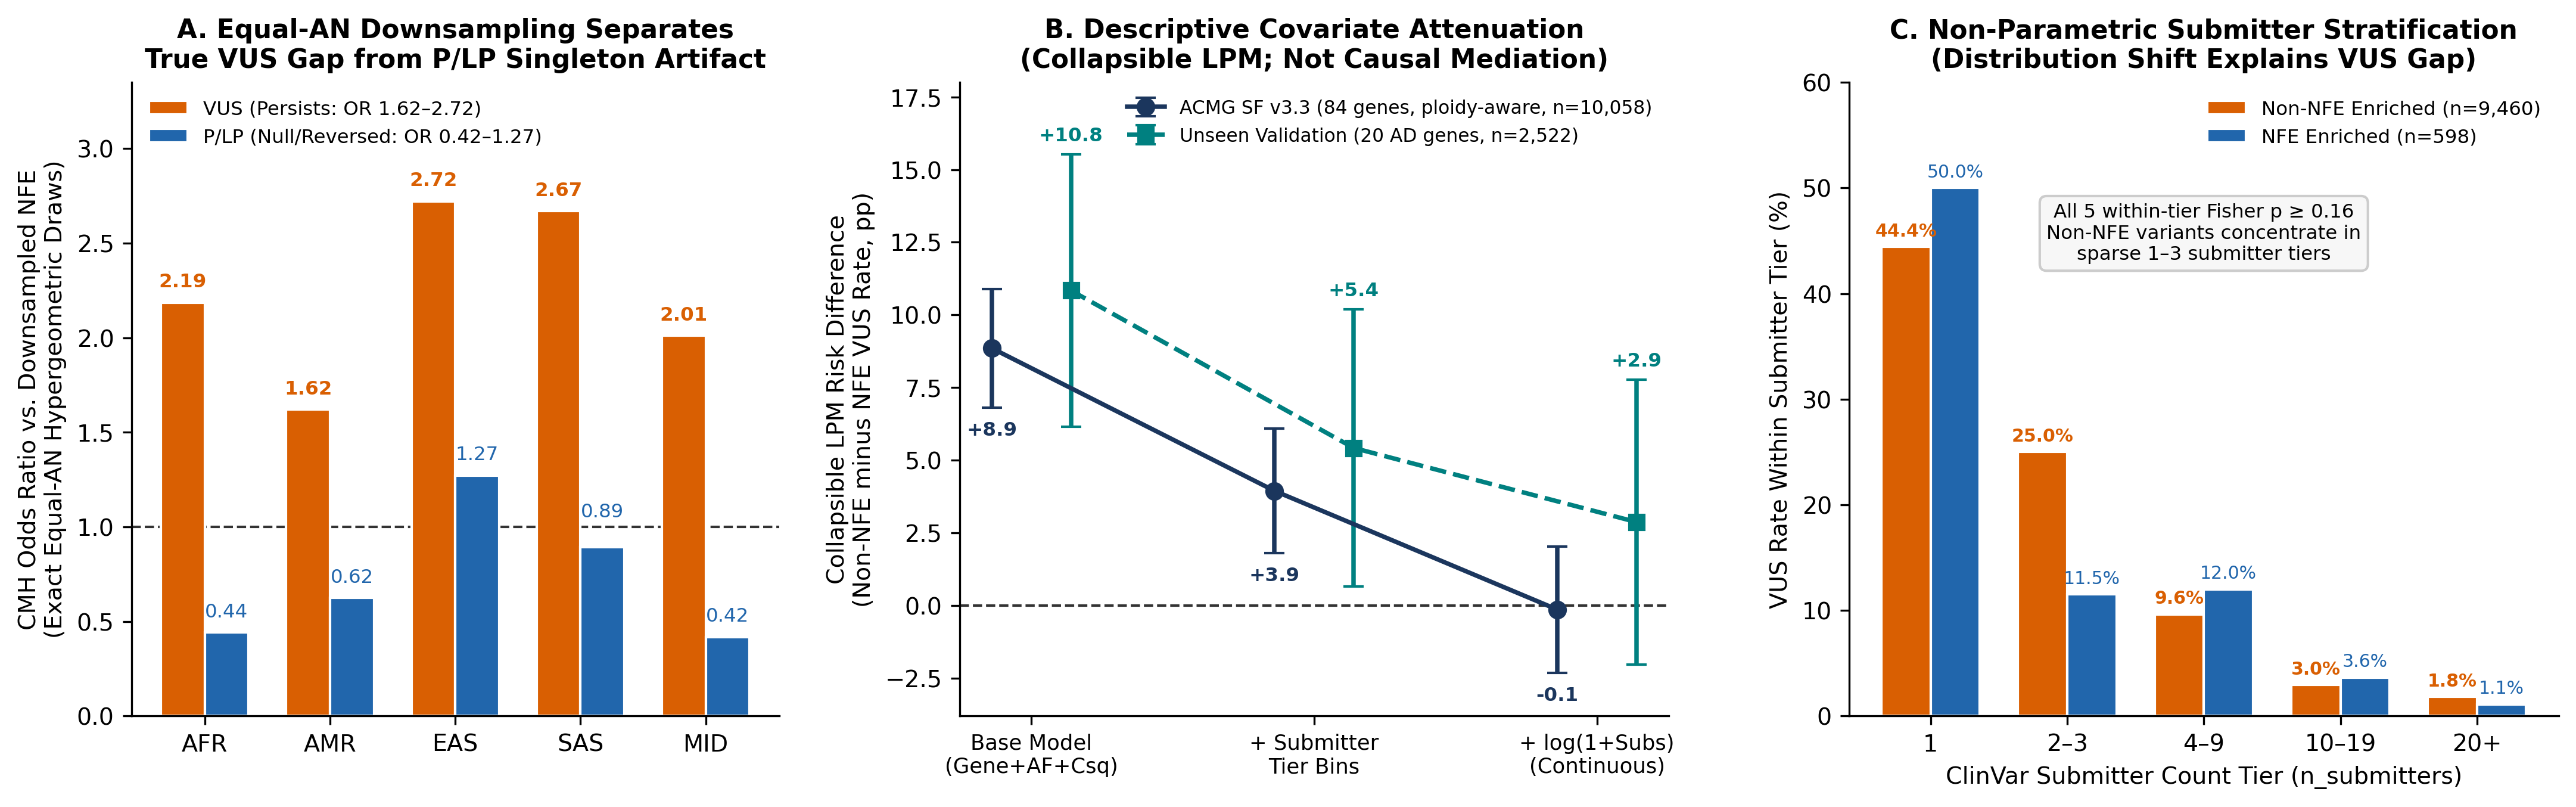
\includegraphics[width=\textwidth]{../figures/fig1_a1_equity_and_curation_velocity.png}
\caption{\textbf{Denominator-Clean Cross-Ancestry VUS Persistence and Descriptive Submitter-Tier Stratification.} (\textbf{A}) Exact equal-AN hypergeometric downsampling separates genuine VUS persistence (OR 1.62--2.72 across all five non-NFE ancestries) from the retracted P/LP singleton artifact (OR 0.42--1.27). (\textbf{B}) Collapsible LPM risk differences across ploidy-aware ACMG SF v3.3 (84 genes, $n=10,058$) and prospective unseen validation (20 AD genes, $n=2,522$) before and after conditioning on submitter tiers or $\log(1+n_{\text{submitters}})$. (\textbf{C}) Within every fixed submitter-count tier, non-NFE and NFE VUS rates are statistically indistinguishable (all Fisher $p\ge 0.16$).}
\label{fig:a1_fig1}
\end{figure}

\subsection{Descriptive Covariate Attenuation Associated with Submission Multiplicity}
Non-NFE-enriched variants carry substantially fewer ClinVar submitters than frequency-matched NFE-enriched variants in both ACMG SF v3.3 (median 7 vs.\ 11) and the unseen 20-gene validation (median 4 vs.\ 8; Mann--Whitney $p=4.05\times 10^{-14}$), and have modestly older evaluation dates ($-0.31$ years adjusted, $p=1.38\times 10^{-4}$; post-2023 share 89.8\% vs.\ 93.0\%). Crucially, non-parametric stratification across five fixed submitter-count tiers in the ploidy-aware 84-gene cohort reveals no statistically significant ancestry gap in VUS rates within any single tier (Figure~\ref{fig:a1_fig1}C; all Fisher $p\ge 0.16$; identical within-tier null contrasts in unseen 20 genes, all $p\ge 0.27$). Rather, non-NFE variants concentrate heavily in sparse 1--3 submitter tiers (22.1\% vs.\ 5.1\% autosomal).

In collapsible LPM regressions adjusting for gene, consequence, and $\mathrm{FAF}_{95}$, conditioning on non-parametric submitter-tier bins descriptively attenuates the VUS risk difference by \textbf{55.5\%} in ploidy-aware ACMG 84 ($+8.86 \to +3.94$ pp, $p=3.24\times 10^{-4}$; autosomal-only 53.0\%, $+9.14 \to +4.29$ pp) and \textbf{50.0\%} in the unseen 20 genes ($+10.84 \to +5.42$ pp, $p=0.026$), while continuous $\log(1+n_{\text{submitters}})$ attenuates the LPM gap to null ($-0.14$ pp, $p=0.899$; unseen 20: $+2.87$ pp, $p=0.251$; autosomal logistic AME 84.5\% attenuation). Because submitter count is an endogenous cross-sectional count jointly shaped by testing volume, variant age, and classification status, these models represent \textbf{descriptive covariate decompositions rather than identified causal mediation} \citep{imai2010mediation,mood2010logistic}.

\subsection{Complete 55/55 AD and X-Linked Live-QC, Official CSpec/Johnston DAFT, and Mode-of-Inheritance Triage}
Live gnomAD v4.1 QC inspection, ClinVar submission-level evidence parsing, and verified CSpec/Johnston 2026 BS1/BA1 evaluation across all 55 allele-exact 2--4$\star$ AD P/LP alerts ($\mathrm{FAF}_{95}\ge 10^{-4}$) yielded \textbf{0 of 55 (0.0\%)} variants exceeding verified gene-specific BA1 and \textbf{0 of 55} unambiguous frequency-only AD P/LP misclassifications (Figure~\ref{fig:a1_fig2}B and Figure~\ref{fig:a1_fig3}):
\begin{itemize}
  \item \textbf{L1 --- Technical QC / Callability Artifacts ($n=8/55$, 14.5\%):} Seven variants had low joint callability ($\mathrm{AN}<80\%$), PLUS one stealth artifact caught only via live gnomAD filter inspection: \textit{APC} \texttt{5-112775626-T-A} (c.423-3T$>$A, 2$\star$, AMR $\mathrm{FAF}_{95}=0.00158$) had 93.9\% AN yet \textbf{failed \texttt{AS\_VQSR} in both exomes and genomes} (\texttt{AC0, AS\_VQSR}).
  \item \textbf{L2 --- European Bottleneck Founders ($n=22/55$, 40.0\%):} Finnish (\texttt{fin}) or Ashkenazi Jewish (\texttt{asj}) founder alleles.
  \item \textbf{L3 --- Established Continental Founders / Low-Penetrance / Pseudogene ($n=14/55$, 25.5\%):} Including \textit{TTR} p.Val142Ile, \textit{APOB} p.Arg3527Gln/Trp, \textit{MYBPC3} p.Arg502Trp, \textit{RET} p.Val804Met, \textit{PMS2} p.Ser46Ile, \textit{RYR1} p.Gly2434Arg, and \textit{PMS2} exon 14 pseudogene homology.
  \item \textbf{L4a --- Genuine AD Pathogenic Alleles Below Verified BS1 ($n=6/55$, 10.9\%):} \textit{LDLR} p.His583Tyr and p.Asp90Asn (\texttt{GN013}), \textit{MYBPC3} c.3330+5G$>$C and p.Arg820Gln (\texttt{GN095}), \textit{KCNQ1} p.Cys122fs (\texttt{GN112}), and \textit{SCN5A} p.Arg225Trp (Johnston 2026 DAFT).
  \item \textbf{L4b --- Autosomal-Recessive-in-AD-Gene Secondary-Finding Return Hazards ($n=4/55$, 7.3\%):} Four live-QC-passed alleles in dual-mode \textit{RYR1}/\textit{TTN} carry unstratified 2--3$\star$ P/LP tags in ClinVar VCFs despite submission-level evidence supporting autosomal recessive myopathy (Table~\ref{tab:a1_l4}): \textit{RYR1} p.Arg3550Trp (SAS AF $0.00167 >$ \texttt{GN012} AD MH BS1 $0.0008$), \textit{RYR1} c.10348-6C$>$G (AFR AF $0.00045$---explicitly designated a pathogenic AR myopathy BA1/BS1 exclusion allele in ClinGen CSpec \texttt{GN179} v2.0), \textit{RYR1} p.Ile2781fs (AFR $0.00020$), and \textit{TTN} p.Lys25729Ter (SAS $\mathrm{FAF}_{95}=0.00015$).
  \item \textbf{L4c --- Reduced-Penetrance Pharmacogenetic Allele Above Johnston DAFT BS1, Below BA1 ($n=1/55$, 1.8\%):} \textit{CACNA1S} p.Arg1086Ser (SAS $\mathrm{FAF}_{95}=0.000218$ vs.\ Johnston DAFT BS1 $0.000050$, BA1 $0.00050$), independently documented in Johnston et al.\ (2026, Table 4) as reflecting uncertain anesthetic-exposure penetrance rather than benign misclassification \citep{johnston2026daft}.
  \item \textbf{X-Linked 2--4$\star$ P/LP Audit (\textit{ABCD1}, \textit{GLA}, \textit{OTC}):} Across all three non-PAR X-linked genes, exactly \textbf{1} 2--4$\star$ P/LP variant has $\mathrm{FAF}_{95}\ge 10^{-4}$ or $\ge$ BS1: \textit{GLA} \texttt{X-101398011-C-T} (2$\star$, AMR $\mathrm{FAF}_{95}=0.000219$, 18 male hemizygotes, live-QC PASS), which remains strictly below Johnston et al.'s combined Fabry/HCM DAFT BS1 ($0.000363$; BA1 $0.003626$).
\end{itemize}

\begin{figure}[H]
\centering
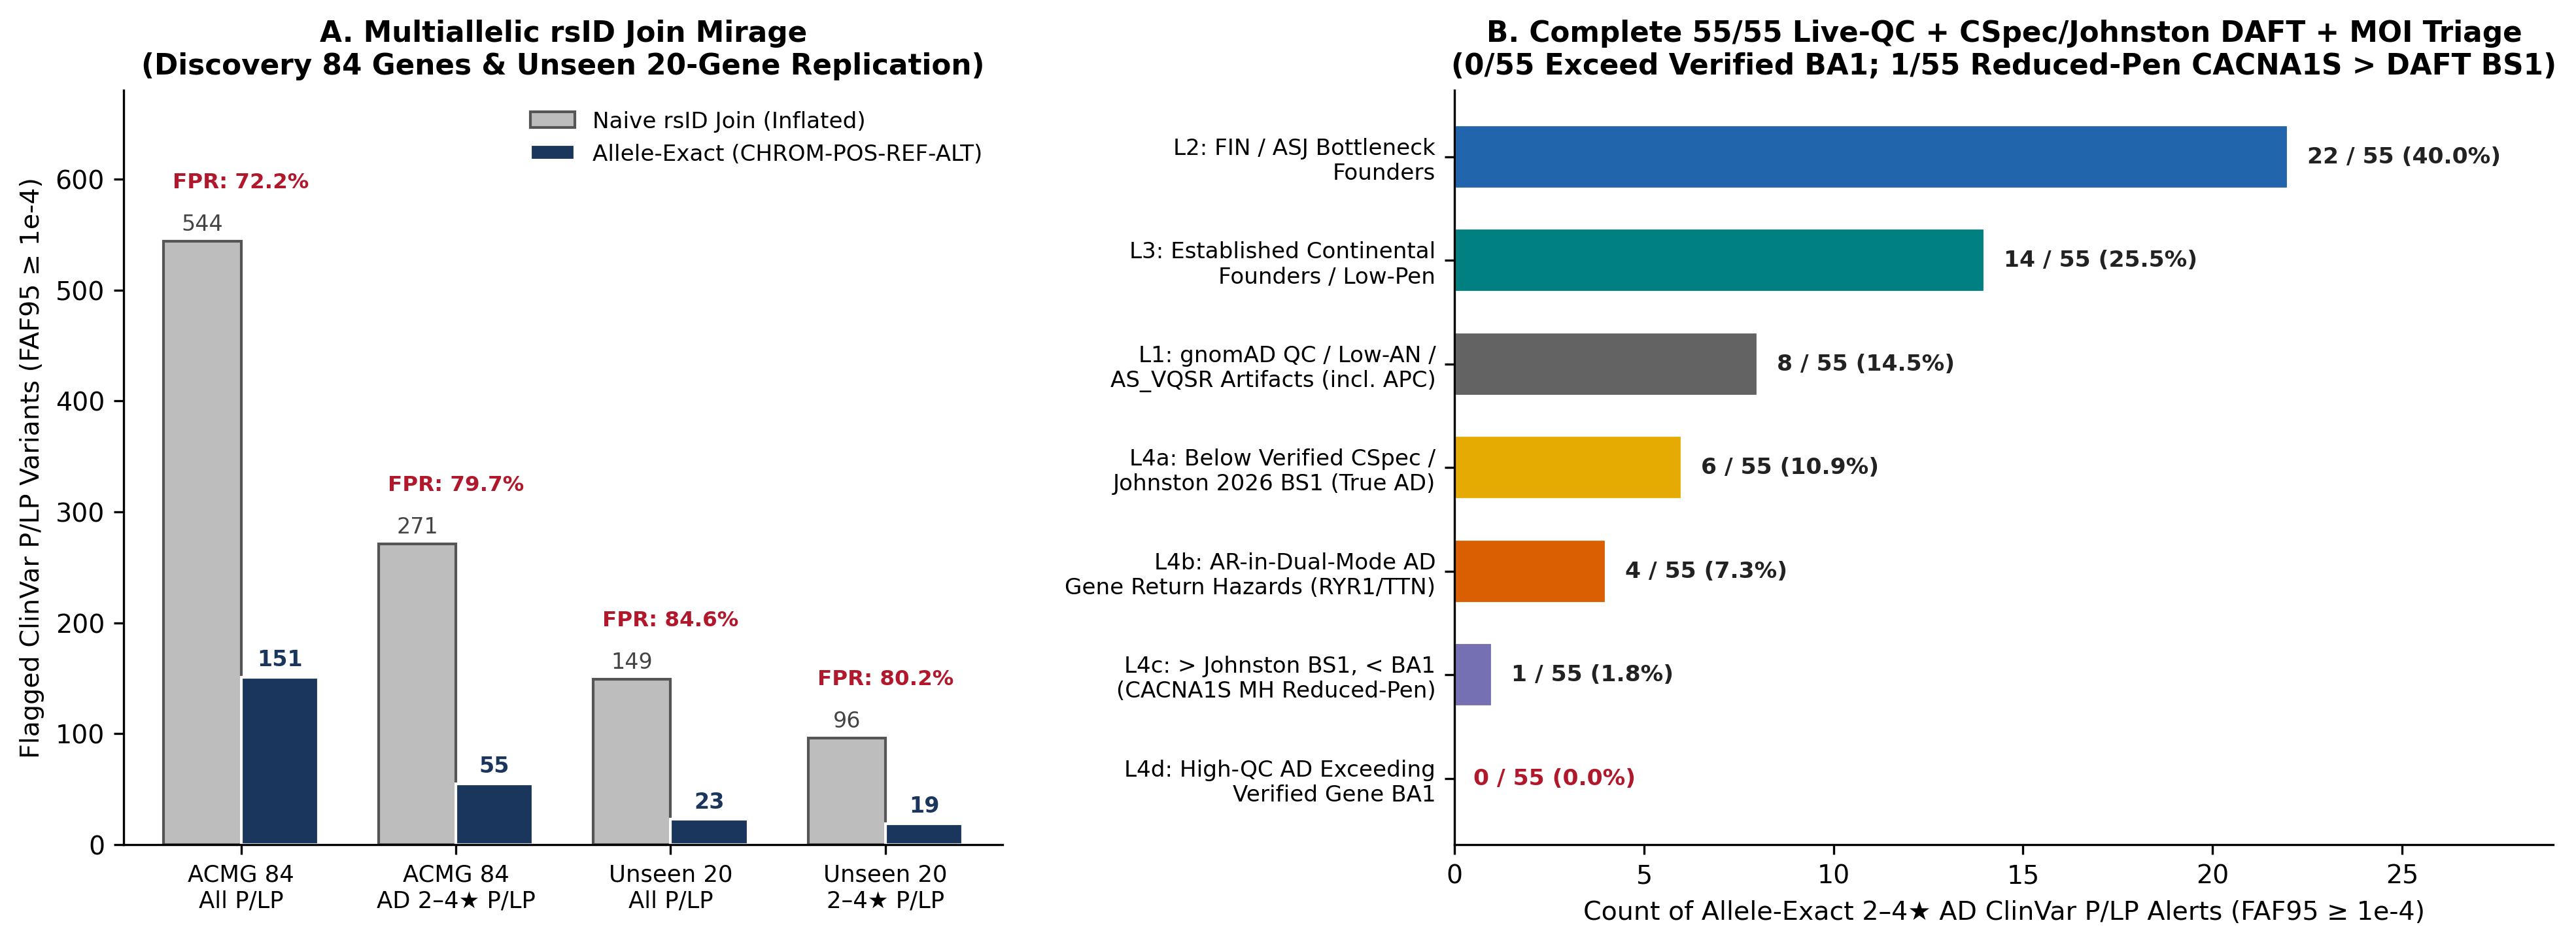
\includegraphics[width=\textwidth]{../figures/fig2_a1_rsid_mirage_and_4layer_triage.png}
\caption{\textbf{Multiallelic rsID Join Inflation and Complete 55/55 Live-QC + CSpec/Johnston DAFT + MOI Triage.} (\textbf{A}) Naive rsID matching inflates $\mathrm{FAF}_{95}\ge 10^{-4}$ P/LP alerts by 72.2\%--84.6\% across ACMG SF v3.3 and unseen 20 AD genes. (\textbf{B}) Exhaustive triage of all 55 allele-exact 2--4$\star$ AD alerts confirms 0/55 above verified BA1 while isolating 8 technical QC artifacts (incl.\ stealth \texttt{AS\_VQSR} fail in \textit{APC}), 4 AR-in-AD return hazards, and 1 reduced-penetrance \textit{CACNA1S} allele exceeding DAFT BS1.}
\label{fig:a1_fig2}
\end{figure}

\begin{table}[H]
\centering
\caption{Complete Audit of All 11 Live-QC-Passed Non-Bottleneck 2--4$\star$ AD P/LP Alerts ($\mathrm{FAF}_{95}\ge 10^{-4}$; \textit{APC} c.423-3T$>$A Excluded as \texttt{AS\_VQSR} Fail) Under Verified ClinGen CSpec \& Johnston (2026) DAFT Thresholds.}
\label{tab:a1_l4}
\scriptsize
\setlength{\tabcolsep}{3.5pt}
\resizebox{\textwidth}{!}{%
\begin{tabular}{llllcccl}
\toprule
\textbf{Gene} & \textbf{Variant (GRCh38)} & \textbf{HGVS / Stars} & \textbf{Pop} & \textbf{Freq$^\dagger$} & \textbf{Verified BS1 (Source)} & \textbf{Hom} & \textbf{Verified Triage Tier} \\
\midrule
\textit{RYR1} & 19-38527014-C-T & p.Arg3550Trp (3$\star$) & SAS & 0.00167 & 0.00080 (\texttt{GN012}) & 0 & L4b: AR-in-AD Return Hazard \\
\textit{RYR1} & 19-38523211-C-G & c.10348-6C$>$G (3$\star$) & AFR & 0.00045 & 0.00080 (\texttt{GN012}$^*$) & 0 & L4b: AR-in-AD Return Hazard \\
\textit{RYR1} & 19-38505338-CAT-C & p.Ile2781fs (2$\star$) & AFR & 0.00020 & 0.00080 (\texttt{GN012}) & 0 & L4b: AR-in-AD Return Hazard \\
\textit{TTN}  & 2-178568947-T-A & p.Lys25729Ter (2$\star$) & SAS & 0.00015 & 0.00130 (Johnston 2026) & 0 & L4b: AR-in-AD Return Hazard \\
\midrule
\textit{CACNA1S} & 1-201060816-G-T & p.Arg1086Ser (2$\star$) & SAS & 0.00022 & 0.00005 (Johnston 2026) & 1 & L4c: $>$ DAFT BS1, $<$ BA1 (MH) \\
\midrule
\textit{LDLR} & 19-11116900-C-T & p.His583Tyr (3$\star$) & EAS & 0.00031 & 0.00200 (\texttt{GN013}) & 1 & L4a: True AD ($<$ CSpec BS1) \\
\textit{KCNQ1} & 11-2445461-A-AT & p.Cys122fs (2$\star$) & SAS & 0.00025 & 0.00040 (\texttt{GN112}) & 0 & L4a: True AD ($<$ CSpec BS1) \\
\textit{MYBPC3} & 11-47333189-C-G & c.3330+5G$>$C (2$\star$) & AFR & 0.00019 & 0.00020 (\texttt{GN095}) & 0 & L4a: True AD ($<$ CSpec BS1) \\
\textit{LDLR} & 19-11102741-G-A & p.Asp90Asn (3$\star$) & EAS & 0.00017 & 0.00200 (\texttt{GN013}) & 0 & L4a: True AD ($<$ CSpec BS1) \\
\textit{MYBPC3} & 11-47337534-C-T & p.Arg820Gln (2$\star$) & EAS & 0.00010 & 0.00020 (\texttt{GN095}) & 0 & L4a: True AD ($<$ CSpec BS1) \\
\textit{SCN5A} & 3-38613773-G-A & p.Arg225Trp (2$\star$) & AFR & 0.00010 & 0.00103 (Johnston 2026) & 1 & L4a: True AD ($<$ DAFT BS1) \\
\bottomrule
\end{tabular}%
}
\\[3pt]\footnotesize{$^\dagger$Rule-faithful continental metric (raw AF for \textit{RYR1} \texttt{GN012} and \textit{KCNQ1} \texttt{GN112}; $\mathrm{FAF}_{95}$ for all others). $^*$\textit{RYR1} c.10348-6C$>$G is explicitly listed as an AR myopathy BA1/BS1 exclusion allele in ClinGen CSpec \texttt{GN179} v2.0.}
\end{table}

\begin{figure}[H]
\centering
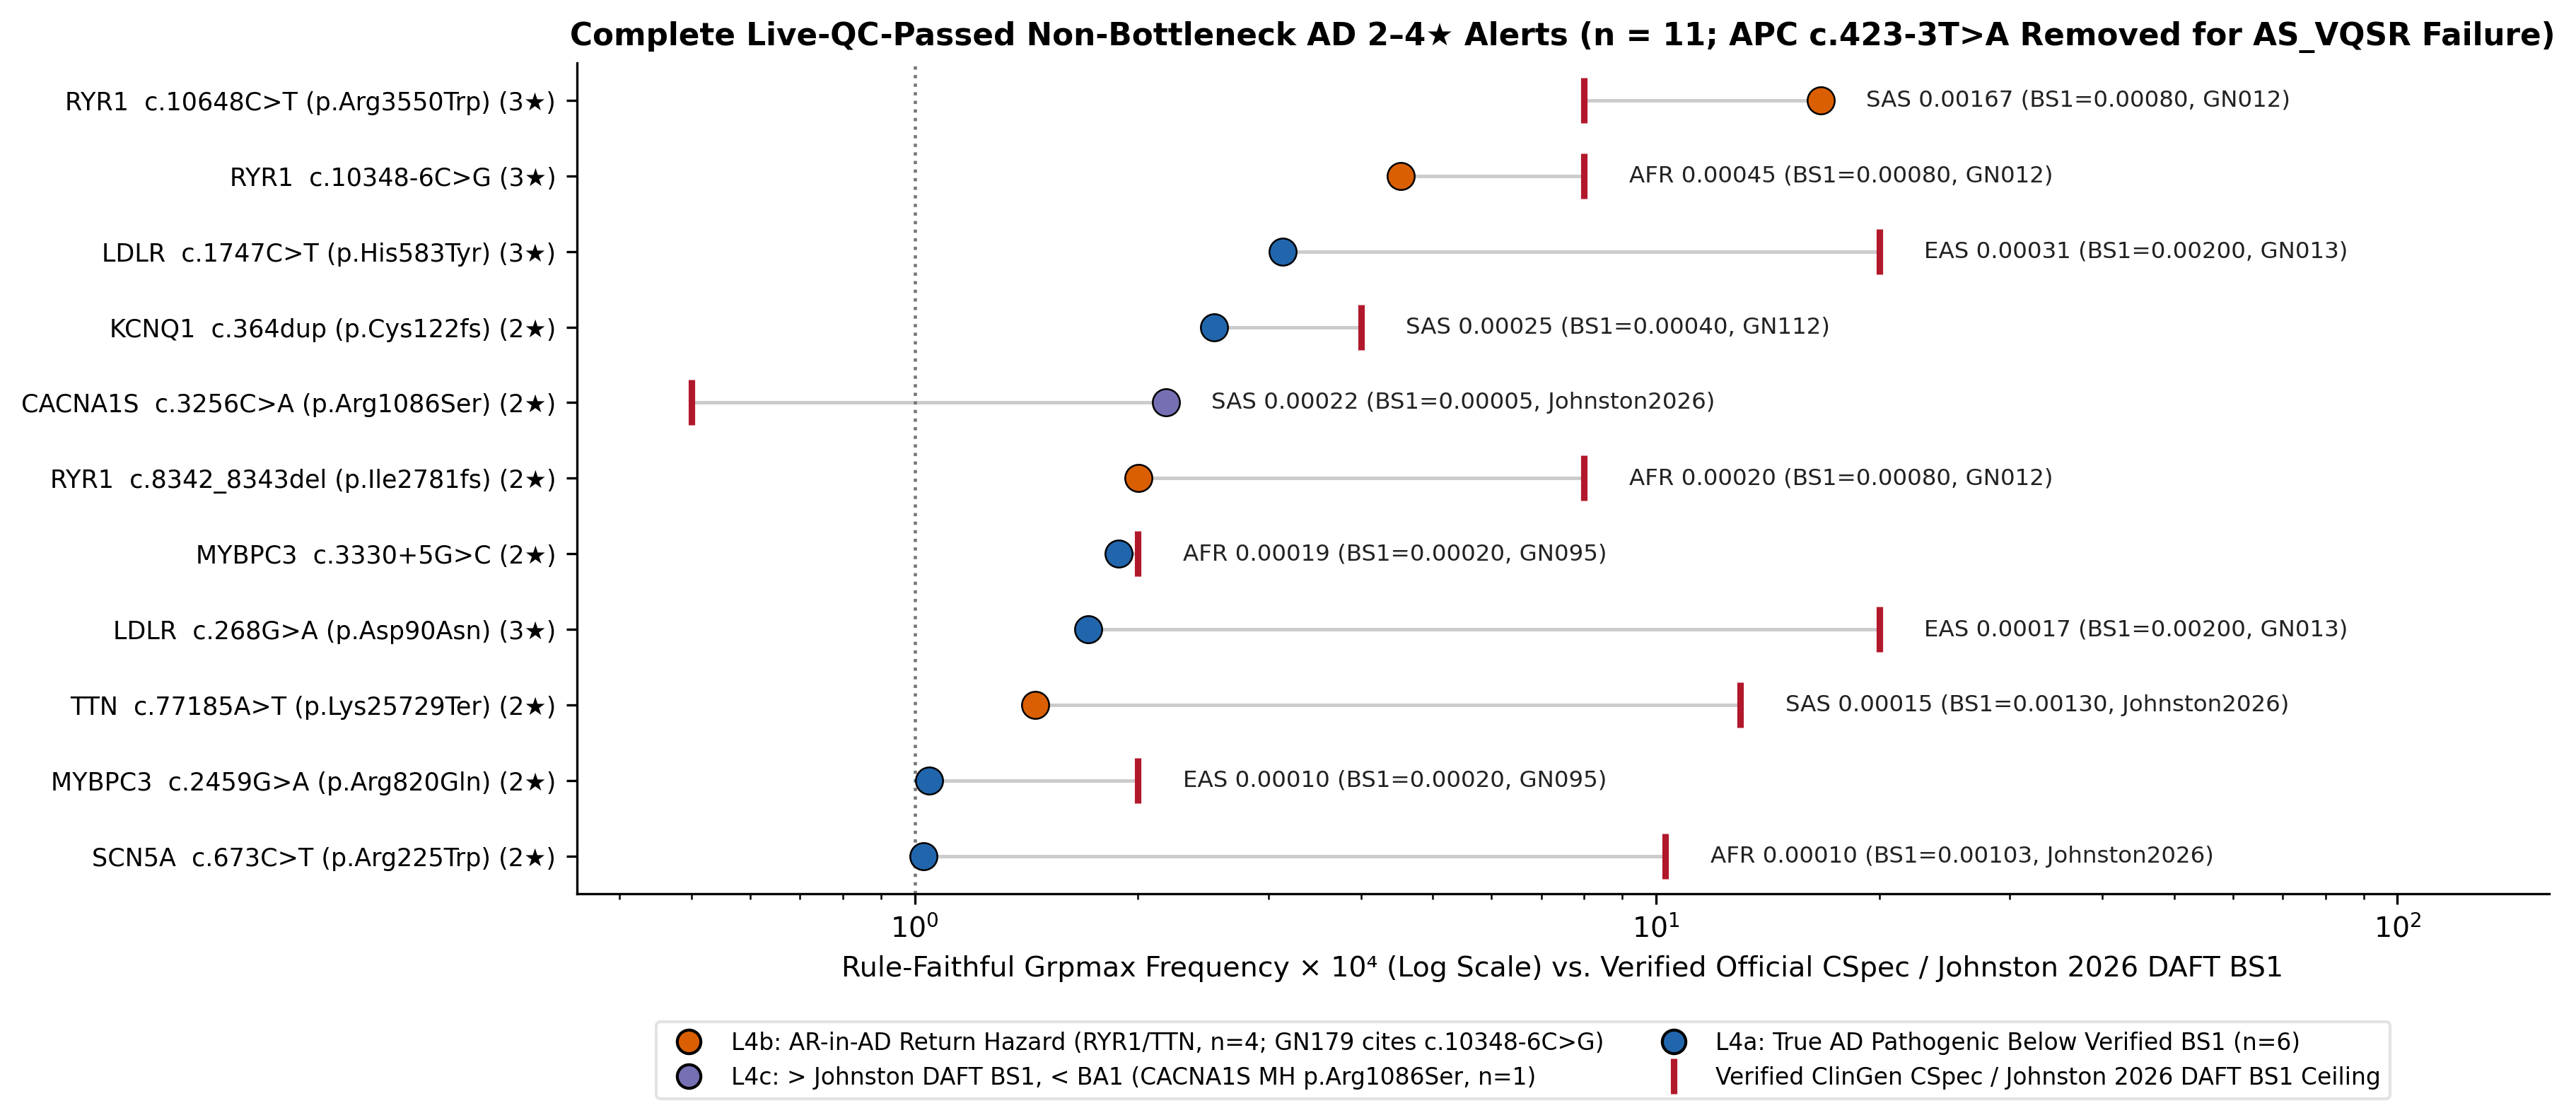
\includegraphics[width=\textwidth]{../figures/fig3_a1_l4_priority_catalog_and_carrier_burden.png}
\caption{\textbf{All 11 Live-QC-Passed Non-Bottleneck AD 2--4$\star$ Alerts Compared Against Official ClinGen CSpec and Johnston et al.\ (2026) DAFT BS1 Ceilings.} Only two variants exceed their AD gene-specific BS1 ceiling: \textit{RYR1} p.Arg3550Trp (a recessive myopathy return hazard) and \textit{CACNA1S} p.Arg1086Ser (a known reduced-penetrance MH allele remaining below BA1 $=0.00050$).}
\label{fig:a1_fig3}
\end{figure}

\subsection{Ploidy-Aware Verified ClinGen CSpec (30 Genes) and Johnston et al.\ (2026) DAFT VUS Queue}
Applying our ploidy-aware 4-tier rule table (excluding \textit{HFE} and named BA1/BS1 exceptions) across all 51,190 high-callability VUS (50,784 autosomal + 406 recovered chrX non-PAR) yields a complete, traceable clinical review queue (Figure~\ref{fig:a1_fig4} and Table~\ref{tab:a1_vus_tiers}):
\begin{itemize}
  \item \textbf{Tier 1 --- 30 Officially Released ClinGen CSpec VCEP Genes (Primary Queue, 18,008 VUS):} \textbf{327 VUS meet official BS1/BA1 criteria} (\textbf{77.7\% NFE-invisible}; 278 with $\mathrm{AC}\ge 5$; 322 frequency-only without the \textit{OTC} hemizygote rule; 247 under uniform $\mathrm{FAF}_{95}$; 320 excluding \textit{BRCA1}/\textit{BRCA2}) and \textbf{21 meet BA1} (\textbf{90.5\% NFE-invisible}), led by \textit{APC} \texttt{GN089} v2.1 ($n=107$), \textit{FBN1} \texttt{GN022} ($n=93$), \textit{HNF1A} \texttt{GN017} ($n=22$), \textit{VHL} \texttt{GN078} ($n=13$), \textit{ABCD1} \texttt{GN105} ($n=11$), \textit{PTEN} \texttt{GN003} ($n=10$), and \textit{OTC} \texttt{GN156} ($n=5$).
  \item \textbf{Recovered chrX Non-PAR VUS Audit (17 Variants, 100\% Live-QC \& Hemizygote Audited):} Correcting the chrX ploidy denominator recovered 17 flagged X-linked VUS: (i) \textbf{11 in \textit{ABCD1}} (\texttt{GN105} v1.0, $\mathrm{BS1}=1.7\times 10^{-5}$, $\mathrm{BA1}=1.7\times 10^{-4}$), including \texttt{X-153729352-G-T} (SAS $\mathrm{FAF}_{95}=0.000276 > \mathrm{BA1}$, 17 male hemizygotes, live-QC PASS), while live QC caught \texttt{X-153743749-G-C} failing \texttt{AS\_VQSR}+\texttt{segdup} and flagged 4 additional exon 7--10 variants with \texttt{segdup} (reflecting known \textit{ABCD1} pseudogene paralogs); (ii) \textbf{5 in \textit{OTC}} (\texttt{GN156} v1.0), all 5 meeting BA1 specifically via the official $\ge 10$ male-hemizygote criterion (12--55 hemizygotes; \texttt{X-38367296-G-A} [55], \texttt{X-38403703-C-G} [48], \texttt{X-38381428-C-T} [AFR, 21], \texttt{X-38369851-C-T} [15], \texttt{X-38381417-C-T} [12]; 5/5 live-QC PASS); and (iii) \textbf{1 in \textit{GLA}} (Tier 3 Johnston DAFT: \texttt{X-101397903-C-G}, SAS $\mathrm{FAF}_{95}=0.000486 > \mathrm{BS1}=0.000363$, 19 male hemizygotes, live-QC PASS).
  \item \textbf{Tier 2 (6 Prelim VCEPs) \& Tier 3 (47 Johnston DAFT Genes):} Tier 2 yields \textbf{99 VUS $\ge$ BS1} (42.4\% NFE-invisible; 76 with $\mathrm{AC}\ge 5$) and \textbf{9 $\ge$ BA1} (77.8\% NFE-invisible); Tier 3 yields \textbf{962 VUS $\ge$ BS1} (48.8\% NFE-invisible; 870 with $\mathrm{AC}\ge 5$) and \textbf{216 $\ge$ BA1} (75.9\% NFE-invisible), led by ultra-low-DAFT \textit{MYH11} ($n=413$) and \textit{WT1} ($n=60$). Across all 83 thresholded genes, \textbf{1,388 VUS meet BS1/BA1} (55.1\% NFE-invisible; 1,224 with $\mathrm{AC}\ge 5$) and \textbf{246 meet BA1} (77.2\% NFE-invisible). Combined live gnomAD QC auditing across 37 VUS candidates (20 stratified autosomal + all 17 chrX) confirmed \textbf{36/37 (97.3\%) PASS} hard filters (the single failure being \textit{ABCD1} \texttt{X-153743749-G-C} \texttt{AS\_VQSR}). Exceeding BS1/BA1 prioritizes variants for formal clinical expert review rather than automatic benign reclassification \citep{richards2015standards,ghosh2018ba1,johnston2026daft}.
\end{itemize}

\begin{table}[H]
\centering
\caption{Ploidy-Aware Tier-Stratified High-Callability VUS Frequency-Conflict Review Queue Under Live ClinGen CSpec (2026-11-25) and Johnston et al.\ (2026) DAFT Thresholds ($n=51,190$ VUS Across 83 Genes; Excl.\ \textit{HFE} \& Named Exceptions).}
\label{tab:a1_vus_tiers}
\scriptsize
\setlength{\tabcolsep}{2pt}
\begin{tabularx}{\textwidth}{>{\raggedright\arraybackslash}X c c c c c c}
\toprule
\textbf{Threshold Tier / Sensitivity} & \textbf{Genes} & \textbf{VUS $\ge$ BS1/BA1} & \textbf{NFE-Invis} & \textbf{VUS $\ge$ BA1} & \textbf{NFE-Invis} & \textbf{BS1 ($\mathrm{AC}\ge 5$)} \\
\midrule
Tier 1: Released CSpec VCEPs (Ploidy-Aware + \textit{OTC} Hemi) & 30 & 327 & 77.7\% & 21 & 90.5\% & 278 (73.7\%) \\
\quad --- Sensitivity: Frequency Threshold Only (Excl.\ \textit{OTC} Hemi) & 30 & 322 & 77.3\% & 16 & 87.5\% & 273 (73.3\%) \\
\quad --- Sensitivity: Uniform Conservative $\mathrm{FAF}_{95}$ Only & 30 & 247 & 72.5\% & 16 & 87.5\% & 227 (70.0\%) \\
\quad --- Sensitivity: Excl.\ \textit{BRCA1}/\textit{BRCA2} Non-Cancer Caveat & 28 & 320 & 77.2\% & 21 & 90.5\% & 271 (73.1\%) \\
Tier 2: Preliminary VCEPs (Johnston 2026 Table 1) & 6 & 99 & 42.4\% & 9 & 77.8\% & 76 (25.0\%) \\
Tier 3: Published DAFT (Johnston 2026 Tables 2--3; incl.\ \textit{GLA}) & 47 & 962 & 48.8\% & 216 & 75.9\% & 870 (43.3\%) \\
\midrule
\textbf{All 83 Thresholded ACMG SF v3.3 Genes (Ploidy-Aware)} & \textbf{83} & \textbf{1,388} & \textbf{55.1\%} & \textbf{246} & \textbf{77.2\%} & \textbf{1,224 (49.1\%)} \\
\bottomrule
\end{tabularx}
\end{table}

\begin{figure}[H]
\centering
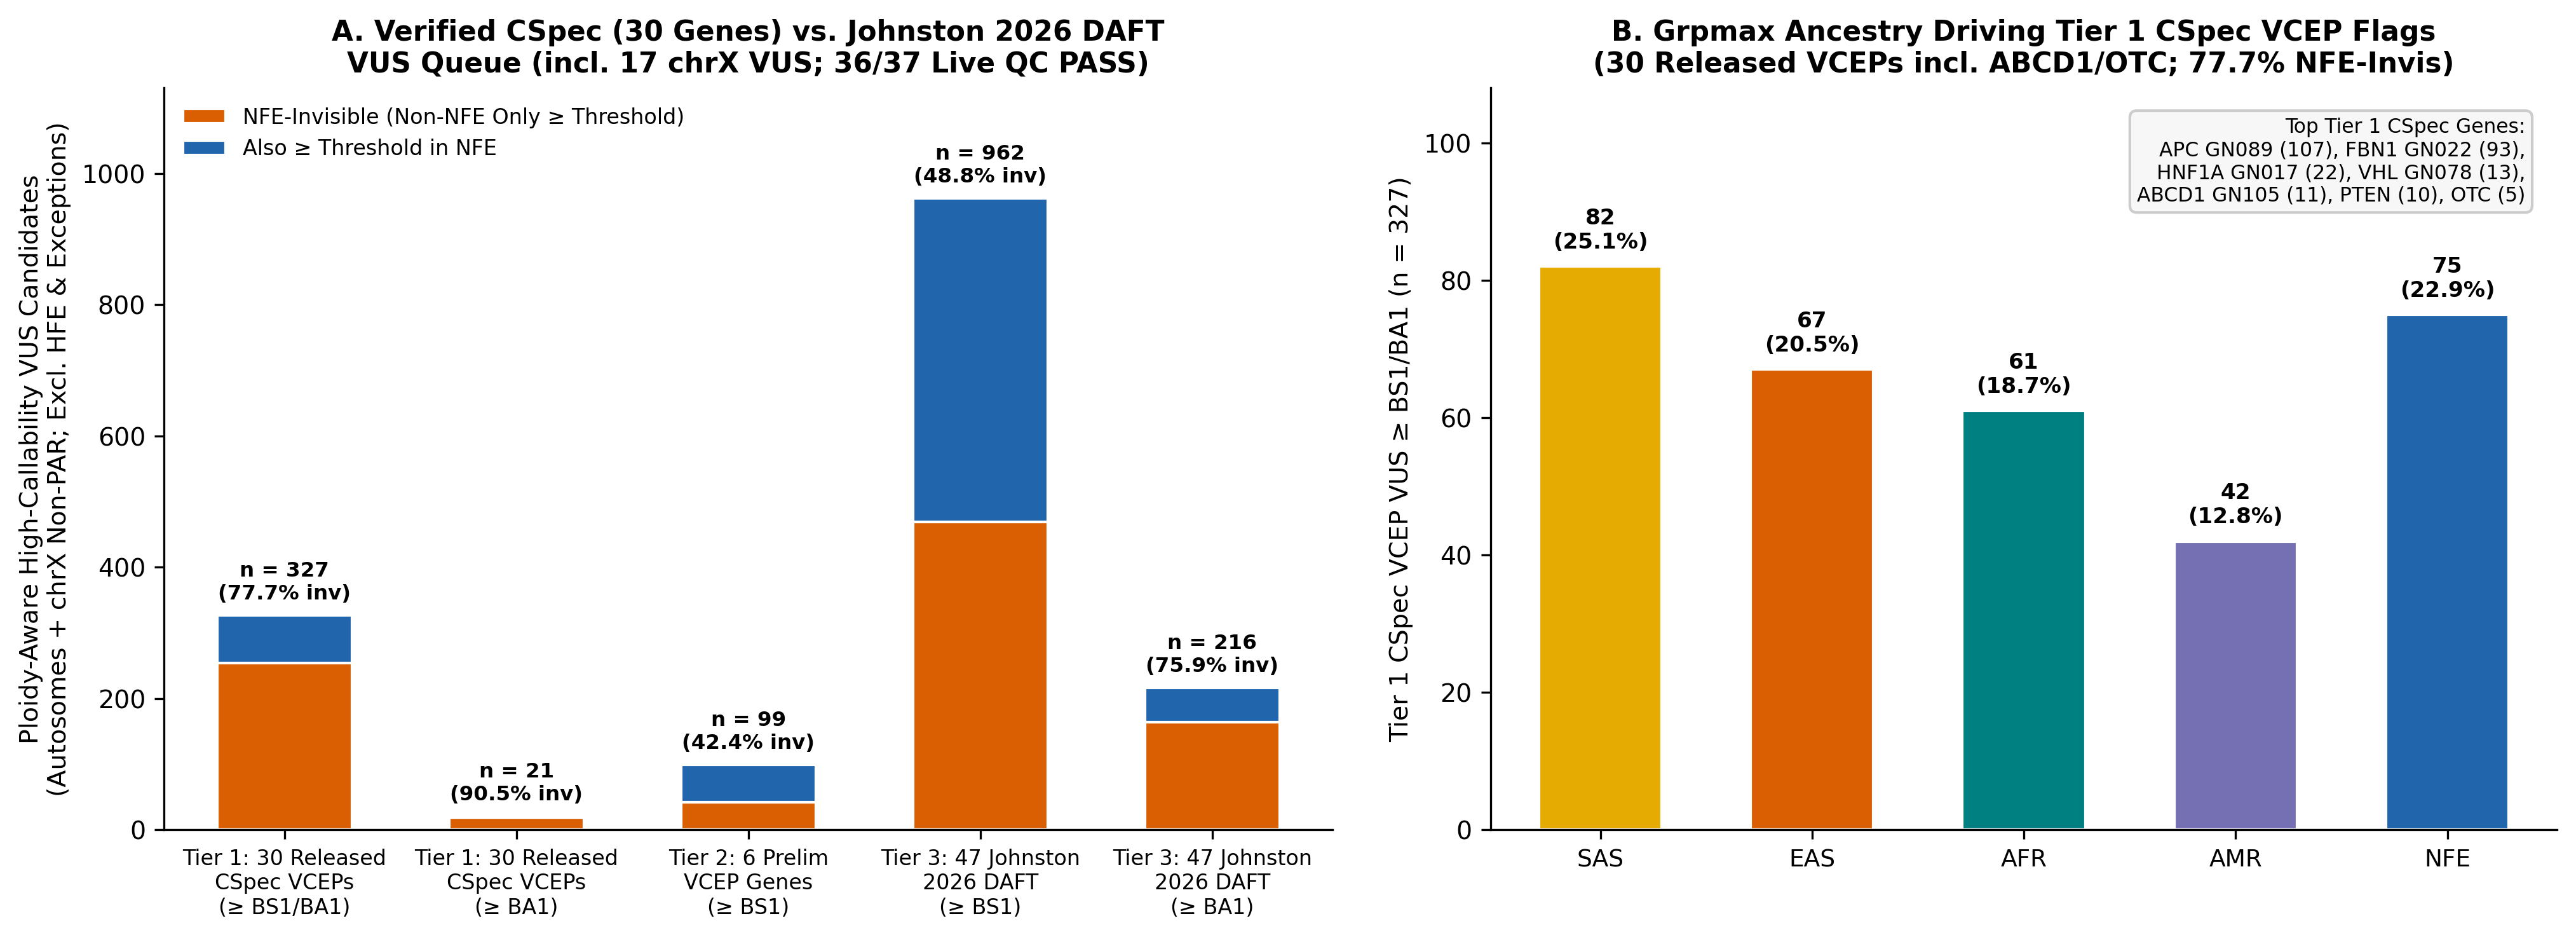
\includegraphics[width=\textwidth]{../figures/fig4_a1_vus_liberation_and_post2024_governance.png}
\caption{\textbf{Ploidy-Aware Verified Official ClinGen CSpec (30 Genes) and Johnston et al.\ (2026) DAFT VUS Frequency-Conflict Queue.} (\textbf{A}) High-callability VUS exceeding verified BS1/BA1 ceilings across Tiers 1--3 including all 17 recovered chrX non-PAR VUS (combined live QC: 36/37 PASS). (\textbf{B}) Grpmax ancestry distribution inside the 30 officially Released ClinGen CSpec VCEP genes ($n=327$, 77.7\% NFE-invisible).}
\label{fig:a1_fig4}
\end{figure}

\section{Discussion and Limitations}
Our findings integrate live 2026 ClinGen CSpec specifications \citep{clingencspec2026}, Johnston et al.'s (2026) secondary-findings DAFT baseline \citep{johnston2026daft}, and ploidy-correct chrX non-PAR callability \citep{gnomadv41sex2024} into an allele-exact, denominator-controlled audit across all 84 ACMG SF v3.3 genes and 20 prospectively locked unseen AD genes. First, high-confidence (2--4$\star$) AD P/LP assertions are far cleaner than naive automated audits imply: after eliminating 72.2\%--79.7\% multiallelic rsID false positives, filtering 8/55 technical QC/callability artifacts (including stealth \texttt{AS\_VQSR} failure in \textit{APC} c.423-3T$>$A), separating 36/55 bottleneck and continental founders, and checking verified CSpec/DAFT ceilings (0/55 above BA1; 1/55 reduced-penetrance \textit{CACNA1S} MH allele above DAFT BS1), zero unambiguous frequency-only AD P/LP misclassifications remain. Instead, the concrete clinical informatics hazard is \textbf{schema-level mode-of-inheritance conflation} in dual-mode \textit{RYR1} and \textit{TTN} (including \textit{RYR1} c.10348-6C$>$G, explicitly designated an AR myopathy exception in ClinGen CSpec \texttt{GN179}), which could be resolved directly by adding mode-of-inheritance tags to ClinVar VCF \texttt{INFO} fields.

Second, our transparent retraction of aggregate raw-AF P/LP disparity and correction of autosomal-vs-chrX ploidy filtering establish two mandatory technical standards for multi-ancestry database audits: equal-AN hypergeometric downsampling (or zero-singleton $\mathrm{FAF}_{95}$) to prevent small-AN singleton bias, and explicit $N_{XY}+2N_{XX}$ denominators with hemizygote extraction on non-PAR chrX (recovering 406 X-linked VUS and 5 \textit{OTC} hemizygote BA1 alerts that autosomal filtering misses entirely). Meanwhile, non-European VUS persistence is robust across every clean test and replicates prospectively in 20 unseen AD genes, tracking concentration in sparse 1--3 submitter tiers. Third, extending Johnston et al.'s (2026) P/LP evaluation to 51,190 high-callability VUS reveals 327 BS1/BA1 (77.7\% NFE-invisible) and 21 BA1 (90.5\% NFE-invisible) candidates strictly inside the 30 officially Released ClinGen CSpec VCEP genes.

\textbf{Limitations:} (1) Two Tier 1 CSpec specifications (\textit{BRCA1} \texttt{GN092}, \textit{BRCA2} \texttt{GN097}) prescribe gnomAD non-cancer subsets; excluding both leaves Tier 1 virtually unchanged (320 vs.\ 327 BS1/BA1; 21 vs.\ 21 BA1). (2) Tier 2 (6 preliminary VCEPs) and Tier 3 (47 Johnston DAFT genes) provide interim guidance pending formal CSpec release, and ultra-low DAFTs (\textit{MYH11}, \textit{WT1}) can trigger BS1 at $\mathrm{AC}<5$; we stratify strictly by tier and report $\mathrm{AC}\ge 5$ sensitivities. (3) Live gnomAD QC filters were verified exhaustively for 55/55 AD P/LP alerts and 18/18 flagged chrX variants (catching 1 \textit{ABCD1} \texttt{AS\_VQSR}+\texttt{segdup} failure and 4 \textit{ABCD1} \texttt{segdup} paralog flags), and via a 20-variant stratified spot-check (20/20 PASS) for autosomal VUS candidates; clinical pipelines should gate every variant on full filter and \texttt{segdup} flags prior to curation. (4) Cross-sectional ClinVar submitter-count adjustments are strictly descriptive and cannot prove causal mediation \citep{imai2010mediation}. (5) This audit evaluates population frequencies and registry metadata rather than patient-level penetrance or functional assays.

\section*{Data and Code Availability}
{\sloppy
All raw ClinVar snapshots, gnomAD v4.1 gene JSON caches, live ClinGen CSpec JSON dumps (\path{audit/cspec_live_acmg84_all_verified.json}), primary-source-verified 84-gene rule tables (\path{audit/a1_acmg84_verified_cspec_johnston2026_rules.csv}, \path{audit/a1_ad55_verified_t05_triage.csv}, \path{audit/a1_vus_verified_t05_t08_bs1_candidates.csv}), chrX ploidy audit (\path{audit/a1_t08_chrx_ploidy_closure.json}), prospective validation lock (\path{PROSPECTIVE_VALIDATION_A1.md}), and runnable scripts are archived in \path{studies/study_a1_clinvar_gnomad_reclass/}.\par}

\bibliographystyle{unsrtnat}
\bibliography{references_a1}
\end{document}
